\newpage
\section{Preuve de Concept : Analyse des Données Augmentées}

\subsection{Introduction}

La réalisation d'une preuve de concept (PoC) \cite{poc} est une importance cruciale dans le contexte de développement d'un modèle de détection de dégradations à partir de données accélérométriques. Cette démarche permet d'évaluer l'utilisabilité des données augmentées avant de pouvoir les déployer dans notre modèle de détection.

Elle permet d'expérimenter et de valider rapidement l'approche envisagée, en utilisant un ensemble initial de données limité. Cette étape préliminaire offre l'opportunité de détecter d'éventuels obstacles techniques, de régler des problèmes spécifiques et d'ajuster la méthodologie, garantissant ainsi une meilleure robustesse du modèle final.

Cette la réalisation d'une preuve de concept dans un projet de détection de dégradations à partir de données accélérométriques contribue à réduire les risques associés au déploiement d'une solution à grande échelle.

\subsection*{Axes et Orientation}

Le repère choisi pour les accélérations est défini comme suit :
\begin{itemize}
    \item Positive X : Avant (Forward)
    \item Positive Y : Gauche (Left)
    \item Positive Z : Haut (Up)
\end{itemize}

\subsection{Analyse des Données}

Deux jeux de données sont examinés : Axe initial ax et Axe inversé ax (donnée augmentée. Tous deux concernent l'accélération selon l'axe des X. Chaque jeu de données est accompagné d'une interprétation. Nous allons nous intéresser plus particulièrement au cas où le robot a rencontré un dos d'âne.

\subsubsection{Initial ax}

\begin{figure}[H]
    \centering
    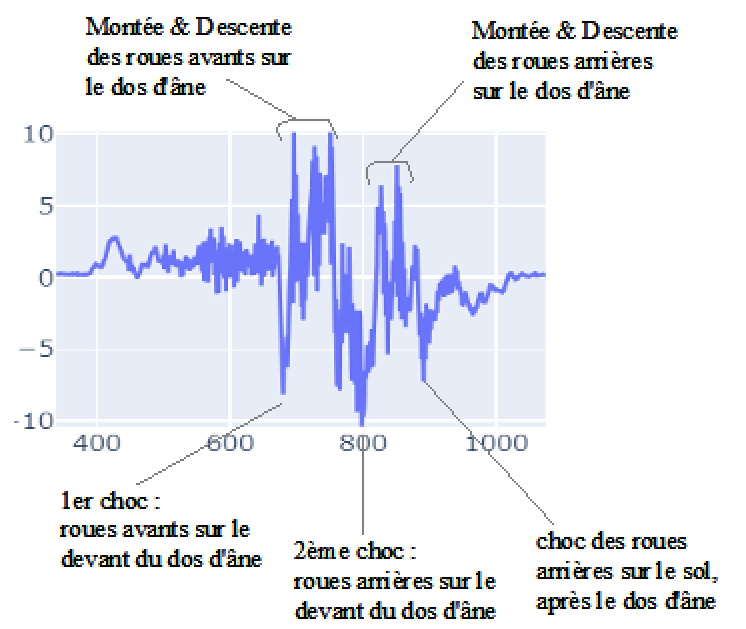
\includegraphics[width=0.5\linewidth]{img/initial_ax.png}
    \caption{Axe ax initial (Zoomé)}
\end{figure}

\textbf{Interprétation :} 
Le robot accélère avant d'arriver au dos d'âne : les chocs des roues avant et arrières se distinguent par des pics importants de valeurs négatifs (ralentissements brutales du robot). Nous remarquons également deux pics de valeurs positifs importants, qui indiquent que le robot réaccélère immédiatement après. La fin de la séquence nous indique que le robot fini par conserver une vitesse stable après avoir passé l'obstacle.

\subsubsection{Inverted ax}

\begin{figure}[H]
    \centering
    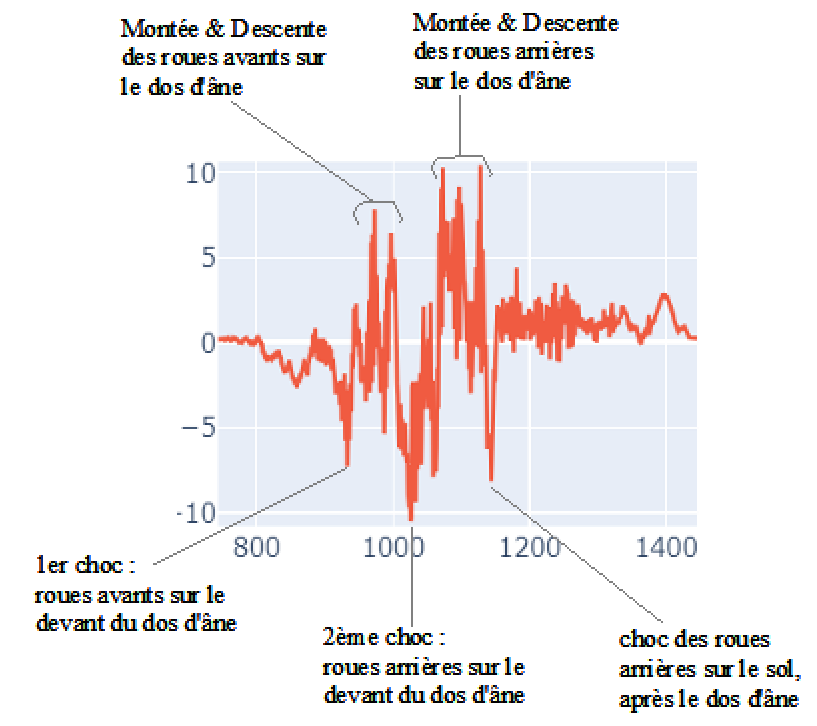
\includegraphics[width=0.5\linewidth]{img/reverted_ax.png}
    \caption{Axe ax inversé dans le temps (Zoomé)}
\end{figure}

\textbf{Interprétation :} 
Le robot semble dans ce cas présent déccelérer avant d'arriver au dos d'âne : l'accélération devient négatif à l'approche du dos d'âne. Les chocs des roues avant et arrières se distinguent par des pics de valeurs négatifs (ralentissements brutales du robot), mais sont moins importants que ceux du signal initial car le robot possède une vitesse moindre. Nous remarquons également deux pics de valeurs positifs importants, qui indiquent que le robot réaccélère dans sa traversée du dodane. La moyenne positive d'environ 3km/h en fin de la séquence nous indique que le robot continue d'accélerer après avoir passer le dos d'âne, contrairement au signal initial.\\


\noindent \textbf{Conclusion}

\noindent L'analyse des différentes configurations d'axes suggère que les données \textit{ax inverted} sont valides pour le dataset. Cette conclusion est basée sur des variations dans le comportement du robot et des différences notables dans les intensités de choc pendant le passage des dos d'âne. Cette preuve de concept s'applique également aux autres opérations cohérentes sur les séquences afin d'obtenir des données augmentées.
